\documentclass[1p]{elsarticle_modified}
%\bibliographystyle{elsarticle-num}

%\usepackage[colorlinks]{hyperref}
%\usepackage{abbrmath_seonhwa} %\Abb, \Ascr, \Acal ,\Abf, \Afrak
\usepackage{amsfonts}
\usepackage{amssymb}
\usepackage{amsmath}
\usepackage{amsthm}
\usepackage{scalefnt}
\usepackage{amsbsy}
\usepackage{kotex}
\usepackage{caption}
\usepackage{subfig}
\usepackage{color}
\usepackage{graphicx}
\usepackage{xcolor} %% white, black, red, green, blue, cyan, magenta, yellow
\usepackage{float}
\usepackage{setspace}
\usepackage{hyperref}

\usepackage{tikz}
\usetikzlibrary{arrows}

\usepackage{multirow}
\usepackage{array} % fixed length table
\usepackage{hhline}

%%%%%%%%%%%%%%%%%%%%%
\makeatletter
\renewcommand*\env@matrix[1][\arraystretch]{%
	\edef\arraystretch{#1}%
	\hskip -\arraycolsep
	\let\@ifnextchar\new@ifnextchar
	\array{*\c@MaxMatrixCols c}}
\makeatother %https://tex.stackexchange.com/questions/14071/how-can-i-increase-the-line-spacing-in-a-matrix
%%%%%%%%%%%%%%%

\usepackage[normalem]{ulem}

\newcommand{\msout}[1]{\ifmmode\text{\sout{\ensuremath{#1}}}\else\sout{#1}\fi}
%SOURCE: \msout is \stkout macro in https://tex.stackexchange.com/questions/20609/strikeout-in-math-mode

\newcommand{\cancel}[1]{
	\ifmmode
	{\color{red}\msout{#1}}
	\else
	{\color{red}\sout{#1}}
	\fi
}

\newcommand{\add}[1]{
	{\color{blue}\uwave{#1}}
}

\newcommand{\replace}[2]{
	\ifmmode
	{\color{red}\msout{#1}}{\color{blue}\uwave{#2}}
	\else
	{\color{red}\sout{#1}}{\color{blue}\uwave{#2}}
	\fi
}

\newcommand{\Sol}{\mathcal{S}} %segment
\newcommand{\D}{D} %diagram
\newcommand{\A}{\mathcal{A}} %arc


%%%%%%%%%%%%%%%%%%%%%%%%%%%%%5 test

\def\sl{\operatorname{\textup{SL}}(2,\Cbb)}
\def\psl{\operatorname{\textup{PSL}}(2,\Cbb)}
\def\quan{\mkern 1mu \triangleright \mkern 1mu}

\theoremstyle{definition}
\newtheorem{thm}{Theorem}[section]
\newtheorem{prop}[thm]{Proposition}
\newtheorem{lem}[thm]{Lemma}
\newtheorem{ques}[thm]{Question}
\newtheorem{cor}[thm]{Corollary}
\newtheorem{defn}[thm]{Definition}
\newtheorem{exam}[thm]{Example}
\newtheorem{rmk}[thm]{Remark}
\newtheorem{alg}[thm]{Algorithm}

\newcommand{\I}{\sqrt{-1}}
\begin{document}

%\begin{frontmatter}
%
%\title{Boundary parabolic representations of knots up to 8 crossings}
%
%%% Group authors per affiliation:
%\author{Yunhi Cho} 
%\address{Department of Mathematics, University of Seoul, Seoul, Korea}
%\ead{yhcho@uos.ac.kr}
%
%
%\author{Seonhwa Kim} %\fnref{s_kim}}
%\address{Center for Geometry and Physics, Institute for Basic Science, Pohang, 37673, Korea}
%\ead{ryeona17@ibs.re.kr}
%
%\author{Hyuk Kim}
%\address{Department of Mathematical Sciences, Seoul National University, Seoul 08826, Korea}
%\ead{hyukkim@snu.ac.kr}
%
%\author{Seokbeom Yoon}
%\address{Department of Mathematical Sciences, Seoul National University, Seoul, 08826,  Korea}
%\ead{sbyoon15@snu.ac.kr}
%
%\begin{abstract}
%We find all boundary parabolic representation of knots up to 8 crossings.
%
%\end{abstract}
%\begin{keyword}
%    \MSC[2010] 57M25 
%\end{keyword}
%
%\end{frontmatter}

%\linenumbers
%\tableofcontents
%
\newcommand\colored[1]{\textcolor{white}{\rule[-0.35ex]{0.8em}{1.4ex}}\kern-0.8em\color{red} #1}%
%\newcommand\colored[1]{\textcolor{white}{ #1}\kern-2.17ex	\textcolor{white}{ #1}\kern-1.81ex	\textcolor{white}{ #1}\kern-2.15ex\color{red}#1	}

{\Large $\underline{12n_{0353}~(K12n_{0353})}$}

\setlength{\tabcolsep}{10pt}
\renewcommand{\arraystretch}{1.6}
\vspace{1cm}\begin{tabular}{m{100pt}>{\centering\arraybackslash}m{274pt}}
\multirow{5}{120pt}{
	\centering
	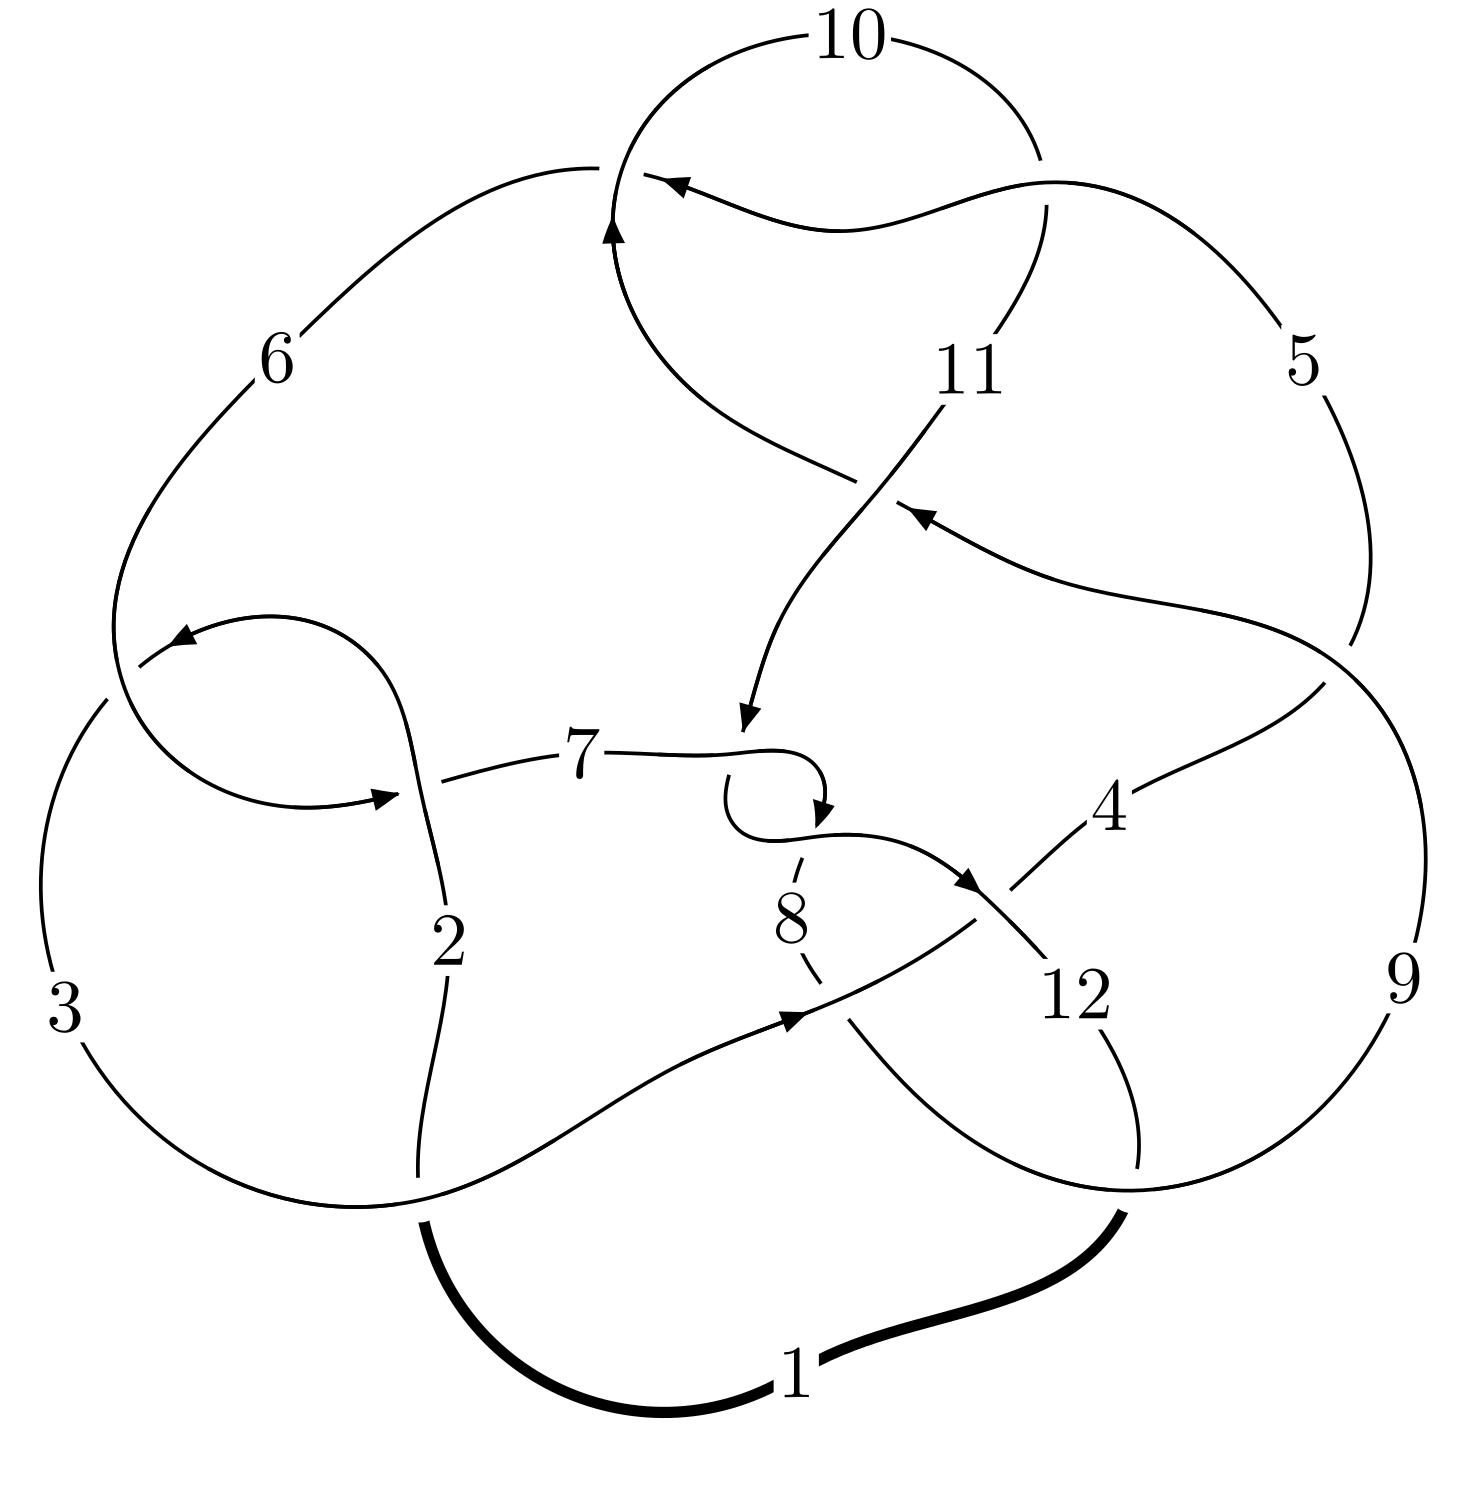
\includegraphics[width=112pt]{../../../GIT/diagram.site/Diagrams/png/2442_12n_0353.png}\\
\ \ \ A knot diagram\footnotemark}&
\allowdisplaybreaks
\textbf{Linearized knot diagam} \\
\cline{2-2}
 &
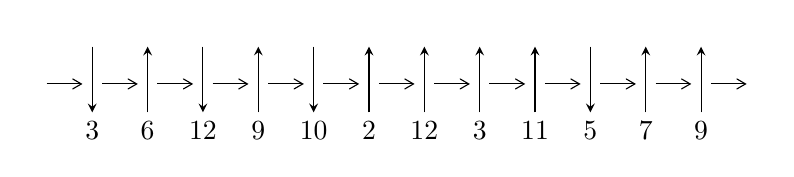
\begin{tikzpicture}[x=20pt, y=17pt]
	% nodes
	\node (C0) at (0, 0) {};
	\node (C1) at (1, 0) {};
	\node (C1U) at (1, +1) {};
	\node (C1D) at (1, -1) {3};

	\node (C2) at (2, 0) {};
	\node (C2U) at (2, +1) {};
	\node (C2D) at (2, -1) {6};

	\node (C3) at (3, 0) {};
	\node (C3U) at (3, +1) {};
	\node (C3D) at (3, -1) {12};

	\node (C4) at (4, 0) {};
	\node (C4U) at (4, +1) {};
	\node (C4D) at (4, -1) {9};

	\node (C5) at (5, 0) {};
	\node (C5U) at (5, +1) {};
	\node (C5D) at (5, -1) {10};

	\node (C6) at (6, 0) {};
	\node (C6U) at (6, +1) {};
	\node (C6D) at (6, -1) {2};

	\node (C7) at (7, 0) {};
	\node (C7U) at (7, +1) {};
	\node (C7D) at (7, -1) {12};

	\node (C8) at (8, 0) {};
	\node (C8U) at (8, +1) {};
	\node (C8D) at (8, -1) {3};

	\node (C9) at (9, 0) {};
	\node (C9U) at (9, +1) {};
	\node (C9D) at (9, -1) {11};

	\node (C10) at (10, 0) {};
	\node (C10U) at (10, +1) {};
	\node (C10D) at (10, -1) {5};

	\node (C11) at (11, 0) {};
	\node (C11U) at (11, +1) {};
	\node (C11D) at (11, -1) {7};

	\node (C12) at (12, 0) {};
	\node (C12U) at (12, +1) {};
	\node (C12D) at (12, -1) {9};
	\node (C13) at (13, 0) {};

	% arrows
	\draw[->,>={angle 60}]
	(C0) edge (C1) (C1) edge (C2) (C2) edge (C3) (C3) edge (C4) (C4) edge (C5) (C5) edge (C6) (C6) edge (C7) (C7) edge (C8) (C8) edge (C9) (C9) edge (C10) (C10) edge (C11) (C11) edge (C12) (C12) edge (C13) ;	\draw[->,>=stealth]
	(C1U) edge (C1D) (C2D) edge (C2U) (C3U) edge (C3D) (C4D) edge (C4U) (C5U) edge (C5D) (C6D) edge (C6U) (C7D) edge (C7U) (C8D) edge (C8U) (C9D) edge (C9U) (C10U) edge (C10D) (C11D) edge (C11U) (C12D) edge (C12U) ;
	\end{tikzpicture} \\
\hhline{~~} \\& 
\textbf{Solving Sequence} \\ \cline{2-2} 
 &
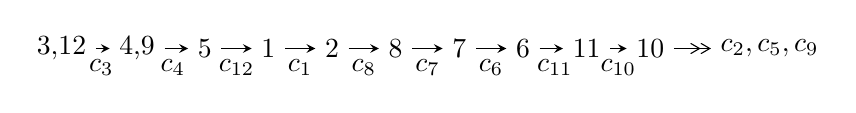
\begin{tikzpicture}[x=23pt, y=7pt]
	% node
	\node (A0) at (-1/8, 0) {3,12};
	\node (A1) at (17/16, 0) {4,9};
	\node (A2) at (17/8, 0) {5};
	\node (A3) at (25/8, 0) {1};
	\node (A4) at (33/8, 0) {2};
	\node (A5) at (41/8, 0) {8};
	\node (A6) at (49/8, 0) {7};
	\node (A7) at (57/8, 0) {6};
	\node (A8) at (65/8, 0) {11};
	\node (A9) at (73/8, 0) {10};
	\node (C1) at (1/2, -1) {$c_{3}$};
	\node (C2) at (13/8, -1) {$c_{4}$};
	\node (C3) at (21/8, -1) {$c_{12}$};
	\node (C4) at (29/8, -1) {$c_{1}$};
	\node (C5) at (37/8, -1) {$c_{8}$};
	\node (C6) at (45/8, -1) {$c_{7}$};
	\node (C7) at (53/8, -1) {$c_{6}$};
	\node (C8) at (61/8, -1) {$c_{11}$};
	\node (C9) at (69/8, -1) {$c_{10}$};
	\node (A10) at (11, 0) {$c_{2},c_{5},c_{9}$};

	% edge
	\draw[->,>=stealth]	
	(A0) edge (A1) (A1) edge (A2) (A2) edge (A3) (A3) edge (A4) (A4) edge (A5) (A5) edge (A6) (A6) edge (A7) (A7) edge (A8) (A8) edge (A9) ;
	\draw[->>,>={angle 60}]	
	(A9) edge (A10);
\end{tikzpicture} \\ 

\end{tabular} \\

\footnotetext{
The image of knot diagram is generated by the software ``\textbf{Draw programme}" developed by Andrew Bartholomew(\url{http://www.layer8.co.uk/maths/draw/index.htm\#Running-draw}), where we modified some parts for our purpose(\url{https://github.com/CATsTAILs/LinksPainter}).
}\phantom \\ \newline 
\centering \textbf{Ideals for irreducible components\footnotemark of $X_{\text{par}}$} 
 
\begin{align*}
I^u_{1}&=\langle 
-9.19698\times10^{252} u^{72}+4.10952\times10^{253} u^{71}+\cdots+1.58931\times10^{253} b+8.73323\times10^{256},\\
\phantom{I^u_{1}}&\phantom{= \langle  }-1.50404\times10^{255} u^{72}+6.27835\times10^{255} u^{71}+\cdots+7.16781\times10^{255} a+2.14004\times10^{259},\\
\phantom{I^u_{1}}&\phantom{= \langle  }u^{73}-4 u^{72}+\cdots-7469 u-4961\rangle \\
I^u_{2}&=\langle 
-9 u^{21}-48 u^{20}+\cdots+b+11,\;28 u^{21}+177 u^{20}+\cdots+a+3,\;u^{22}+7 u^{21}+\cdots+7 u+1\rangle \\
\\
\end{align*}
\raggedright * 2 irreducible components of $\dim_{\mathbb{C}}=0$, with total 95 representations.\\
\footnotetext{All coefficients of polynomials are rational numbers. But the coefficients are sometimes approximated in decimal forms when there is not enough margin.}
\newpage
\renewcommand{\arraystretch}{1}
\centering \section*{I. $I^u_{1}= \langle -9.20\times10^{252} u^{72}+4.11\times10^{253} u^{71}+\cdots+1.59\times10^{253} b+8.73\times10^{256},\;-1.50\times10^{255} u^{72}+6.28\times10^{255} u^{71}+\cdots+7.17\times10^{255} a+2.14\times10^{259},\;u^{73}-4 u^{72}+\cdots-7469 u-4961 \rangle$}
\flushleft \textbf{(i) Arc colorings}\\
\begin{tabular}{m{7pt} m{180pt} m{7pt} m{180pt} }
\flushright $a_{3}=$&$\begin{pmatrix}1\\0\end{pmatrix}$ \\
\flushright $a_{12}=$&$\begin{pmatrix}0\\u\end{pmatrix}$ \\
\flushright $a_{4}=$&$\begin{pmatrix}1\\u^2\end{pmatrix}$ \\
\flushright $a_{9}=$&$\begin{pmatrix}0.209833 u^{72}-0.875910 u^{71}+\cdots+2329.47 u-2985.62\\0.578676 u^{72}-2.58572 u^{71}+\cdots+2145.74 u-5494.97\end{pmatrix}$ \\
\flushright $a_{5}=$&$\begin{pmatrix}-1.50718 u^{72}+6.92175 u^{71}+\cdots-2293.79 u+12596.8\\0.676487 u^{72}-3.11685 u^{71}+\cdots+970.426 u-5595.66\end{pmatrix}$ \\
\flushright $a_{1}=$&$\begin{pmatrix}-0.754050 u^{72}+3.46435 u^{71}+\cdots-1139.08 u+6262.26\\-1.15917 u^{72}+5.32183 u^{71}+\cdots-1731.26 u+9700.40\end{pmatrix}$ \\
\flushright $a_{2}=$&$\begin{pmatrix}0.405124 u^{72}-1.85748 u^{71}+\cdots+592.184 u-3438.14\\-1.15917 u^{72}+5.32183 u^{71}+\cdots-1731.26 u+9700.40\end{pmatrix}$ \\
\flushright $a_{8}=$&$\begin{pmatrix}-0.368843 u^{72}+1.70981 u^{71}+\cdots+183.722 u+2509.35\\0.578676 u^{72}-2.58572 u^{71}+\cdots+2145.74 u-5494.97\end{pmatrix}$ \\
\flushright $a_{7}=$&$\begin{pmatrix}-0.368843 u^{72}+1.70981 u^{71}+\cdots+183.722 u+2509.35\\0.423437 u^{72}-1.87140 u^{71}+\cdots+2066.92 u-4331.94\end{pmatrix}$ \\
\flushright $a_{6}=$&$\begin{pmatrix}-0.0556736 u^{72}+0.215818 u^{71}+\cdots-1052.76 u+687.535\\-0.208916 u^{72}+1.01482 u^{71}+\cdots+1183.76 u+1059.07\end{pmatrix}$ \\
\flushright $a_{11}=$&$\begin{pmatrix}-1.57181 u^{72}+7.22423 u^{71}+\cdots-2235.05 u+13095.6\\0.607582 u^{72}-2.79839 u^{71}+\cdots+843.580 u-5009.04\end{pmatrix}$ \\
\flushright $a_{10}=$&$\begin{pmatrix}-1.51645 u^{72}+7.01530 u^{71}+\cdots-1132.33 u+11925.2\\1.75380 u^{72}-7.99846 u^{71}+\cdots+4270.33 u-15380.1\end{pmatrix}$\\&\end{tabular}
\flushleft \textbf{(ii) Obstruction class $= -1$}\\~\\
\flushleft \textbf{(iii) Cusp Shapes $= 5.97688 u^{72}-27.3063 u^{71}+\cdots+12628.2 u-52558.5$}\\~\\
\newpage\renewcommand{\arraystretch}{1}
\flushleft \textbf{(iv) u-Polynomials at the component}\newline \\
\begin{tabular}{m{50pt}|m{274pt}}
Crossings & \hspace{64pt}u-Polynomials at each crossing \\
\hline $$\begin{aligned}c_{1}\end{aligned}$$&$\begin{aligned}
&u^{73}+42 u^{72}+\cdots+u-1
\end{aligned}$\\
\hline $$\begin{aligned}c_{2},c_{6}\end{aligned}$$&$\begin{aligned}
&u^{73}-2 u^{72}+\cdots+3 u-1
\end{aligned}$\\
\hline $$\begin{aligned}c_{3}\end{aligned}$$&$\begin{aligned}
&u^{73}-4 u^{72}+\cdots-7469 u-4961
\end{aligned}$\\
\hline $$\begin{aligned}c_{4}\end{aligned}$$&$\begin{aligned}
&u^{73}+u^{72}+\cdots+504 u-34447
\end{aligned}$\\
\hline $$\begin{aligned}c_{5},c_{10}\end{aligned}$$&$\begin{aligned}
&u^{73}- u^{72}+\cdots+6 u-19
\end{aligned}$\\
\hline $$\begin{aligned}c_{7},c_{11}\end{aligned}$$&$\begin{aligned}
&u^{73}-3 u^{72}+\cdots+518 u-77
\end{aligned}$\\
\hline $$\begin{aligned}c_{8}\end{aligned}$$&$\begin{aligned}
&u^{73}- u^{72}+\cdots-4184 u-2449
\end{aligned}$\\
\hline $$\begin{aligned}c_{9}\end{aligned}$$&$\begin{aligned}
&u^{73}-35 u^{72}+\cdots-3270 u+361
\end{aligned}$\\
\hline $$\begin{aligned}c_{12}\end{aligned}$$&$\begin{aligned}
&u^{73}+u^{72}+\cdots+9112 u-2479
\end{aligned}$\\
\hline
\end{tabular}\\~\\
\newpage\renewcommand{\arraystretch}{1}
\flushleft \textbf{(v) Riley Polynomials at the component}\newline \\
\begin{tabular}{m{50pt}|m{274pt}}
Crossings & \hspace{64pt}Riley Polynomials at each crossing \\
\hline $$\begin{aligned}c_{1}\end{aligned}$$&$\begin{aligned}
&y^{73}-6 y^{72}+\cdots+109 y-1
\end{aligned}$\\
\hline $$\begin{aligned}c_{2},c_{6}\end{aligned}$$&$\begin{aligned}
&y^{73}+42 y^{72}+\cdots+y-1
\end{aligned}$\\
\hline $$\begin{aligned}c_{3}\end{aligned}$$&$\begin{aligned}
&y^{73}-80 y^{72}+\cdots+887378547 y-24611521
\end{aligned}$\\
\hline $$\begin{aligned}c_{4}\end{aligned}$$&$\begin{aligned}
&y^{73}-5 y^{72}+\cdots+9963979872 y-1186595809
\end{aligned}$\\
\hline $$\begin{aligned}c_{5},c_{10}\end{aligned}$$&$\begin{aligned}
&y^{73}+35 y^{72}+\cdots-3270 y-361
\end{aligned}$\\
\hline $$\begin{aligned}c_{7},c_{11}\end{aligned}$$&$\begin{aligned}
&y^{73}-25 y^{72}+\cdots-47222 y-5929
\end{aligned}$\\
\hline $$\begin{aligned}c_{8}\end{aligned}$$&$\begin{aligned}
&y^{73}+83 y^{72}+\cdots-316258558 y-5997601
\end{aligned}$\\
\hline $$\begin{aligned}c_{9}\end{aligned}$$&$\begin{aligned}
&y^{73}+15 y^{72}+\cdots-1105302 y-130321
\end{aligned}$\\
\hline $$\begin{aligned}c_{12}\end{aligned}$$&$\begin{aligned}
&y^{73}+79 y^{72}+\cdots-157637734 y-6145441
\end{aligned}$\\
\hline
\end{tabular}\\~\\
\newpage\flushleft \textbf{(vi) Complex Volumes and Cusp Shapes}
$$\begin{array}{c|c|c}  
\text{Solutions to }I^u_{1}& \I (\text{vol} + \sqrt{-1}CS) & \text{Cusp shape}\\
 \hline 
\begin{aligned}
u &= \phantom{-}0.960694 + 0.223002 I \\
a &= -0.31701 - 1.62689 I \\
b &= -0.06752 - 1.93464 I\end{aligned}
 & -5.68153 + 1.21562 I & \phantom{-0.000000 } 0 \\ \hline\begin{aligned}
u &= \phantom{-}0.960694 - 0.223002 I \\
a &= -0.31701 + 1.62689 I \\
b &= -0.06752 + 1.93464 I\end{aligned}
 & -5.68153 - 1.21562 I & \phantom{-0.000000 } 0 \\ \hline\begin{aligned}
u &= -0.800102 + 0.544363 I \\
a &= -1.340300 - 0.231886 I \\
b &= -0.229015 + 0.678752 I\end{aligned}
 & \phantom{-}3.32889 + 1.44969 I & \phantom{-0.000000 } 0 \\ \hline\begin{aligned}
u &= -0.800102 - 0.544363 I \\
a &= -1.340300 + 0.231886 I \\
b &= -0.229015 - 0.678752 I\end{aligned}
 & \phantom{-}3.32889 - 1.44969 I & \phantom{-0.000000 } 0 \\ \hline\begin{aligned}
u &= \phantom{-}0.164338 + 1.072630 I \\
a &= -0.568772 + 0.453403 I \\
b &= \phantom{-}0.067159 - 0.480853 I\end{aligned}
 & \phantom{-}3.93954 + 2.04644 I & \phantom{-0.000000 } 0 \\ \hline\begin{aligned}
u &= \phantom{-}0.164338 - 1.072630 I \\
a &= -0.568772 - 0.453403 I \\
b &= \phantom{-}0.067159 + 0.480853 I\end{aligned}
 & \phantom{-}3.93954 - 2.04644 I & \phantom{-0.000000 } 0 \\ \hline\begin{aligned}
u &= -0.436988 + 1.059720 I \\
a &= -0.333172 + 0.259820 I \\
b &= -0.045424 + 0.670574 I\end{aligned}
 & \phantom{-}0.65478 + 1.74378 I & \phantom{-0.000000 } 0 \\ \hline\begin{aligned}
u &= -0.436988 - 1.059720 I \\
a &= -0.333172 - 0.259820 I \\
b &= -0.045424 - 0.670574 I\end{aligned}
 & \phantom{-}0.65478 - 1.74378 I & \phantom{-0.000000 } 0 \\ \hline\begin{aligned}
u &= -0.795078 + 0.220539 I \\
a &= -1.98401 - 0.60795 I \\
b &= -0.300669 - 0.679598 I\end{aligned}
 & \phantom{-}1.18619 - 7.05030 I & \phantom{-0.000000 } 0 \\ \hline\begin{aligned}
u &= -0.795078 - 0.220539 I \\
a &= -1.98401 + 0.60795 I \\
b &= -0.300669 + 0.679598 I\end{aligned}
 & \phantom{-}1.18619 + 7.05030 I & \phantom{-0.000000 } 0\\
 \hline 
 \end{array}$$\newpage$$\begin{array}{c|c|c}  
\text{Solutions to }I^u_{1}& \I (\text{vol} + \sqrt{-1}CS) & \text{Cusp shape}\\
 \hline 
\begin{aligned}
u &= -0.802130 + 0.134868 I \\
a &= -0.306467 + 0.314014 I \\
b &= -0.350471 - 0.748878 I\end{aligned}
 & -3.45310 + 2.18113 I & \phantom{-0.000000 } 0 \\ \hline\begin{aligned}
u &= -0.802130 - 0.134868 I \\
a &= -0.306467 - 0.314014 I \\
b &= -0.350471 + 0.748878 I\end{aligned}
 & -3.45310 - 2.18113 I & \phantom{-0.000000 } 0 \\ \hline\begin{aligned}
u &= -0.330029 + 1.180410 I \\
a &= \phantom{-}0.607699 - 0.317572 I \\
b &= \phantom{-}0.032457 - 0.739244 I\end{aligned}
 & \phantom{-}2.70715 - 2.50353 I & \phantom{-0.000000 } 0 \\ \hline\begin{aligned}
u &= -0.330029 - 1.180410 I \\
a &= \phantom{-}0.607699 + 0.317572 I \\
b &= \phantom{-}0.032457 + 0.739244 I\end{aligned}
 & \phantom{-}2.70715 + 2.50353 I & \phantom{-0.000000 } 0 \\ \hline\begin{aligned}
u &= -0.661879 + 1.045090 I \\
a &= \phantom{-}0.806091 + 0.004427 I \\
b &= \phantom{-}0.145525 - 0.713654 I\end{aligned}
 & \phantom{-}3.77152 + 3.96149 I & \phantom{-0.000000 } 0 \\ \hline\begin{aligned}
u &= -0.661879 - 1.045090 I \\
a &= \phantom{-}0.806091 - 0.004427 I \\
b &= \phantom{-}0.145525 + 0.713654 I\end{aligned}
 & \phantom{-}3.77152 - 3.96149 I & \phantom{-0.000000 } 0 \\ \hline\begin{aligned}
u &= \phantom{-}0.716179 + 0.098392 I \\
a &= \phantom{-}0.780594 - 0.817015 I \\
b &= -0.982012 - 0.581986 I\end{aligned}
 & \phantom{-}4.73461 + 4.33640 I & \phantom{-0.000000 } 0 \\ \hline\begin{aligned}
u &= \phantom{-}0.716179 - 0.098392 I \\
a &= \phantom{-}0.780594 + 0.817015 I \\
b &= -0.982012 + 0.581986 I\end{aligned}
 & \phantom{-}4.73461 - 4.33640 I & \phantom{-0.000000 } 0 \\ \hline\begin{aligned}
u &= \phantom{-}0.632663 + 0.312150 I \\
a &= \phantom{-}1.67667 - 0.35481 I \\
b &= -0.283393 + 0.257017 I\end{aligned}
 & \phantom{-}5.10442 + 3.75309 I & \phantom{-0.000000 } 0 \\ \hline\begin{aligned}
u &= \phantom{-}0.632663 - 0.312150 I \\
a &= \phantom{-}1.67667 + 0.35481 I \\
b &= -0.283393 - 0.257017 I\end{aligned}
 & \phantom{-}5.10442 - 3.75309 I & \phantom{-0.000000 } 0\\
 \hline 
 \end{array}$$\newpage$$\begin{array}{c|c|c}  
\text{Solutions to }I^u_{1}& \I (\text{vol} + \sqrt{-1}CS) & \text{Cusp shape}\\
 \hline 
\begin{aligned}
u &= -0.697508 + 0.042276 I \\
a &= \phantom{-}0.320190 + 1.056290 I \\
b &= \phantom{-}1.293460 + 0.457104 I\end{aligned}
 & \phantom{-}3.08996 + 0.50335 I & \phantom{-0.000000 } 0 \\ \hline\begin{aligned}
u &= -0.697508 - 0.042276 I \\
a &= \phantom{-}0.320190 - 1.056290 I \\
b &= \phantom{-}1.293460 - 0.457104 I\end{aligned}
 & \phantom{-}3.08996 - 0.50335 I & \phantom{-0.000000 } 0 \\ \hline\begin{aligned}
u &= -1.344490 + 0.232038 I \\
a &= \phantom{-}0.222248 + 0.421654 I \\
b &= \phantom{-}0.107848 + 1.300160 I\end{aligned}
 & -3.26184 - 1.83723 I & \phantom{-0.000000 } 0 \\ \hline\begin{aligned}
u &= -1.344490 - 0.232038 I \\
a &= \phantom{-}0.222248 - 0.421654 I \\
b &= \phantom{-}0.107848 - 1.300160 I\end{aligned}
 & -3.26184 + 1.83723 I & \phantom{-0.000000 } 0 \\ \hline\begin{aligned}
u &= -0.629638 + 0.051553 I \\
a &= -0.506953 + 0.948183 I \\
b &= -1.270960 - 0.116190 I\end{aligned}
 & -0.96981 + 3.12263 I & \phantom{-0.000000 } 0. - 3.92838 I \\ \hline\begin{aligned}
u &= -0.629638 - 0.051553 I \\
a &= -0.506953 - 0.948183 I \\
b &= -1.270960 + 0.116190 I\end{aligned}
 & -0.96981 - 3.12263 I & \phantom{-0.000000 -}0. + 3.92838 I \\ \hline\begin{aligned}
u &= \phantom{-}0.623255 + 0.102892 I \\
a &= \phantom{-}0.812430 + 0.004182 I \\
b &= -1.051920 - 0.163847 I\end{aligned}
 & \phantom{-}4.88061 + 4.25358 I & \phantom{-}7.95219 - 6.27359 I \\ \hline\begin{aligned}
u &= \phantom{-}0.623255 - 0.102892 I \\
a &= \phantom{-}0.812430 - 0.004182 I \\
b &= -1.051920 + 0.163847 I\end{aligned}
 & \phantom{-}4.88061 - 4.25358 I & \phantom{-}7.95219 + 6.27359 I \\ \hline\begin{aligned}
u &= -0.570164 + 0.021414 I \\
a &= \phantom{-}0.589757 - 1.092380 I \\
b &= \phantom{-}1.64229 + 0.16254 I\end{aligned}
 & \phantom{-}1.88323 + 7.93272 I & \phantom{-}1.77664 - 7.45810 I \\ \hline\begin{aligned}
u &= -0.570164 - 0.021414 I \\
a &= \phantom{-}0.589757 + 1.092380 I \\
b &= \phantom{-}1.64229 - 0.16254 I\end{aligned}
 & \phantom{-}1.88323 - 7.93272 I & \phantom{-}1.77664 + 7.45810 I\\
 \hline 
 \end{array}$$\newpage$$\begin{array}{c|c|c}  
\text{Solutions to }I^u_{1}& \I (\text{vol} + \sqrt{-1}CS) & \text{Cusp shape}\\
 \hline 
\begin{aligned}
u &= -0.30805 + 1.39618 I \\
a &= \phantom{-}0.292611 + 0.126630 I \\
b &= \phantom{-}0.015318 + 0.602025 I\end{aligned}
 & -0.08107 + 3.31791 I & \phantom{-0.000000 } 0 \\ \hline\begin{aligned}
u &= -0.30805 - 1.39618 I \\
a &= \phantom{-}0.292611 - 0.126630 I \\
b &= \phantom{-}0.015318 - 0.602025 I\end{aligned}
 & -0.08107 - 3.31791 I & \phantom{-0.000000 } 0 \\ \hline\begin{aligned}
u &= -1.38600 + 0.44020 I \\
a &= \phantom{-}0.082384 - 0.995509 I \\
b &= -0.47298 - 1.51710 I\end{aligned}
 & \phantom{-}0.98783 + 1.74704 I & \phantom{-0.000000 } 0 \\ \hline\begin{aligned}
u &= -1.38600 - 0.44020 I \\
a &= \phantom{-}0.082384 + 0.995509 I \\
b &= -0.47298 + 1.51710 I\end{aligned}
 & \phantom{-}0.98783 - 1.74704 I & \phantom{-0.000000 } 0 \\ \hline\begin{aligned}
u &= \phantom{-}1.46506 + 0.00570 I \\
a &= -0.244949 + 0.905533 I \\
b &= \phantom{-}0.06859 + 1.83552 I\end{aligned}
 & -4.04293 - 0.08034 I & \phantom{-0.000000 } 0 \\ \hline\begin{aligned}
u &= \phantom{-}1.46506 - 0.00570 I \\
a &= -0.244949 - 0.905533 I \\
b &= \phantom{-}0.06859 - 1.83552 I\end{aligned}
 & -4.04293 + 0.08034 I & \phantom{-0.000000 } 0 \\ \hline\begin{aligned}
u &= -0.445112 + 0.281624 I \\
a &= \phantom{-}2.64254 + 1.30726 I \\
b &= \phantom{-}0.326600 + 0.664261 I\end{aligned}
 & -0.18113 - 2.12200 I & \phantom{-0.000000 -}     -6
0. 10   + 0.246955 I \\ \hline\begin{aligned}
u &= -0.445112 - 0.281624 I \\
a &= \phantom{-}2.64254 - 1.30726 I \\
b &= \phantom{-}0.326600 - 0.664261 I\end{aligned}
 & -0.18113 + 2.12200 I & \phantom{-0.000000 }      -6
0. 10   - 0.246955 I \\ \hline\begin{aligned}
u &= \phantom{-}1.37711 + 0.55990 I \\
a &= -0.543341 - 1.220170 I \\
b &= -0.10757 - 1.80567 I\end{aligned}
 & -7.78936 - 4.71097 I & \phantom{-0.000000 } 0 \\ \hline\begin{aligned}
u &= \phantom{-}1.37711 - 0.55990 I \\
a &= -0.543341 + 1.220170 I \\
b &= -0.10757 + 1.80567 I\end{aligned}
 & -7.78936 + 4.71097 I & \phantom{-0.000000 } 0\\
 \hline 
 \end{array}$$\newpage$$\begin{array}{c|c|c}  
\text{Solutions to }I^u_{1}& \I (\text{vol} + \sqrt{-1}CS) & \text{Cusp shape}\\
 \hline 
\begin{aligned}
u &= \phantom{-}0.503647\phantom{ +0.000000I} \\
a &= -0.984699\phantom{ +0.000000I} \\
b &= \phantom{-}0.808330\phantom{ +0.000000I}\end{aligned}
 & \phantom{-}1.57161\phantom{ +0.000000I} & \phantom{-}5.96450\phantom{ +0.000000I} \\ \hline\begin{aligned}
u &= \phantom{-}0.463701 + 0.131323 I \\
a &= -1.78260 + 1.42853 I \\
b &= \phantom{-}0.591813 + 0.515091 I\end{aligned}
 & \phantom{-}1.58882 - 0.32095 I & \phantom{-}2.16231 - 0.77182 I \\ \hline\begin{aligned}
u &= \phantom{-}0.463701 - 0.131323 I \\
a &= -1.78260 - 1.42853 I \\
b &= \phantom{-}0.591813 - 0.515091 I\end{aligned}
 & \phantom{-}1.58882 + 0.32095 I & \phantom{-}2.16231 + 0.77182 I \\ \hline\begin{aligned}
u &= \phantom{-}1.48212 + 0.39520 I \\
a &= \phantom{-}0.466011 + 1.151950 I \\
b &= \phantom{-}0.06640 + 1.79340 I\end{aligned}
 & -9.37134 + 0.19549 I & \phantom{-0.000000 } 0 \\ \hline\begin{aligned}
u &= \phantom{-}1.48212 - 0.39520 I \\
a &= \phantom{-}0.466011 - 1.151950 I \\
b &= \phantom{-}0.06640 - 1.79340 I\end{aligned}
 & -9.37134 - 0.19549 I & \phantom{-0.000000 } 0 \\ \hline\begin{aligned}
u &= -0.14949 + 1.54080 I \\
a &= -0.489674 - 0.086157 I \\
b &= -0.047121 - 0.560015 I\end{aligned}
 & \phantom{-}1.51048 + 8.25732 I & \phantom{-0.000000 } 0 \\ \hline\begin{aligned}
u &= -0.14949 - 1.54080 I \\
a &= -0.489674 + 0.086157 I \\
b &= -0.047121 + 0.560015 I\end{aligned}
 & \phantom{-}1.51048 - 8.25732 I & \phantom{-0.000000 } 0 \\ \hline\begin{aligned}
u &= \phantom{-}1.56042 + 0.34674 I \\
a &= \phantom{-}0.010384 - 1.048110 I \\
b &= \phantom{-}0.67684 - 1.68437 I\end{aligned}
 & -1.26128 - 7.24457 I & \phantom{-0.000000 } 0 \\ \hline\begin{aligned}
u &= \phantom{-}1.56042 - 0.34674 I \\
a &= \phantom{-}0.010384 + 1.048110 I \\
b &= \phantom{-}0.67684 + 1.68437 I\end{aligned}
 & -1.26128 + 7.24457 I & \phantom{-0.000000 } 0 \\ \hline\begin{aligned}
u &= \phantom{-}1.65389 + 0.09304 I \\
a &= \phantom{-}0.414399 + 0.961671 I \\
b &= -0.02065 + 1.74832 I\end{aligned}
 & -8.67096 + 2.54106 I & \phantom{-0.000000 } 0\\
 \hline 
 \end{array}$$\newpage$$\begin{array}{c|c|c}  
\text{Solutions to }I^u_{1}& \I (\text{vol} + \sqrt{-1}CS) & \text{Cusp shape}\\
 \hline 
\begin{aligned}
u &= \phantom{-}1.65389 - 0.09304 I \\
a &= \phantom{-}0.414399 - 0.961671 I \\
b &= -0.02065 - 1.74832 I\end{aligned}
 & -8.67096 - 2.54106 I & \phantom{-0.000000 } 0 \\ \hline\begin{aligned}
u &= -0.010648 + 0.336630 I \\
a &= -0.862000 + 0.884016 I \\
b &= \phantom{-}0.186715 + 0.375985 I\end{aligned}
 & \phantom{-}0.391751 + 1.001410 I & \phantom{-}6.35526 - 6.56819 I \\ \hline\begin{aligned}
u &= -0.010648 - 0.336630 I \\
a &= -0.862000 - 0.884016 I \\
b &= \phantom{-}0.186715 - 0.375985 I\end{aligned}
 & \phantom{-}0.391751 - 1.001410 I & \phantom{-}6.35526 + 6.56819 I \\ \hline\begin{aligned}
u &= \phantom{-}1.69732 + 0.15917 I \\
a &= -0.038668 + 1.110620 I \\
b &= \phantom{-}0.55120 + 1.40451 I\end{aligned}
 & -7.69355 - 0.16950 I & \phantom{-0.000000 } 0 \\ \hline\begin{aligned}
u &= \phantom{-}1.69732 - 0.15917 I \\
a &= -0.038668 - 1.110620 I \\
b &= \phantom{-}0.55120 - 1.40451 I\end{aligned}
 & -7.69355 + 0.16950 I & \phantom{-0.000000 } 0 \\ \hline\begin{aligned}
u &= \phantom{-}1.71266 + 0.01894 I \\
a &= -0.436259 + 0.898448 I \\
b &= \phantom{-}0.05204 + 1.71503 I\end{aligned}
 & -6.53777 - 7.64853 I & \phantom{-0.000000 } 0 \\ \hline\begin{aligned}
u &= \phantom{-}1.71266 - 0.01894 I \\
a &= -0.436259 - 0.898448 I \\
b &= \phantom{-}0.05204 - 1.71503 I\end{aligned}
 & -6.53777 + 7.64853 I & \phantom{-0.000000 } 0 \\ \hline\begin{aligned}
u &= -1.64149 + 0.52671 I \\
a &= -0.146618 + 0.979002 I \\
b &= \phantom{-}0.32106 + 1.60321 I\end{aligned}
 & -3.98213 + 4.52901 I & \phantom{-0.000000 } 0 \\ \hline\begin{aligned}
u &= -1.64149 - 0.52671 I \\
a &= -0.146618 - 0.979002 I \\
b &= \phantom{-}0.32106 - 1.60321 I\end{aligned}
 & -3.98213 - 4.52901 I & \phantom{-0.000000 } 0 \\ \hline\begin{aligned}
u &= -1.62388 + 0.66255 I \\
a &= \phantom{-}0.156149 - 1.005480 I \\
b &= -0.33974 - 1.66999 I\end{aligned}
 & -1.69099 + 9.76232 I & \phantom{-0.000000 } 0\\
 \hline 
 \end{array}$$\newpage$$\begin{array}{c|c|c}  
\text{Solutions to }I^u_{1}& \I (\text{vol} + \sqrt{-1}CS) & \text{Cusp shape}\\
 \hline 
\begin{aligned}
u &= -1.62388 - 0.66255 I \\
a &= \phantom{-}0.156149 + 1.005480 I \\
b &= -0.33974 + 1.66999 I\end{aligned}
 & -1.69099 - 9.76232 I & \phantom{-0.000000 } 0 \\ \hline\begin{aligned}
u &= -1.75783 + 0.13522 I \\
a &= -0.154026 + 0.860113 I \\
b &= \phantom{-}0.14670 + 1.46011 I\end{aligned}
 & -5.44293 + 1.91638 I & \phantom{-0.000000 } 0 \\ \hline\begin{aligned}
u &= -1.75783 - 0.13522 I \\
a &= -0.154026 - 0.860113 I \\
b &= \phantom{-}0.14670 - 1.46011 I\end{aligned}
 & -5.44293 - 1.91638 I & \phantom{-0.000000 } 0 \\ \hline\begin{aligned}
u &= \phantom{-}1.77611 + 0.03947 I \\
a &= \phantom{-}0.016455 + 1.094850 I \\
b &= -0.54064 + 1.51324 I\end{aligned}
 & -8.82927 - 5.92695 I & \phantom{-0.000000 } 0 \\ \hline\begin{aligned}
u &= \phantom{-}1.77611 - 0.03947 I \\
a &= \phantom{-}0.016455 - 1.094850 I \\
b &= -0.54064 - 1.51324 I\end{aligned}
 & -8.82927 + 5.92695 I & \phantom{-0.000000 } 0 \\ \hline\begin{aligned}
u &= -1.80292 + 0.06963 I \\
a &= \phantom{-}0.205300 + 0.777815 I \\
b &= -0.03434 + 1.45649 I\end{aligned}
 & -4.37924 + 2.95785 I & \phantom{-0.000000 } 0 \\ \hline\begin{aligned}
u &= -1.80292 - 0.06963 I \\
a &= \phantom{-}0.205300 - 0.777815 I \\
b &= -0.03434 - 1.45649 I\end{aligned}
 & -4.37924 - 2.95785 I & \phantom{-0.000000 } 0 \\ \hline\begin{aligned}
u &= \phantom{-}1.75562 + 0.45978 I \\
a &= -0.028610 + 1.074530 I \\
b &= -0.55514 + 1.73413 I\end{aligned}
 & -7.12058 - 10.34450 I & \phantom{-0.000000 } 0 \\ \hline\begin{aligned}
u &= \phantom{-}1.75562 - 0.45978 I \\
a &= -0.028610 - 1.074530 I \\
b &= -0.55514 - 1.73413 I\end{aligned}
 & -7.12058 + 10.34450 I & \phantom{-0.000000 } 0 \\ \hline\begin{aligned}
u &= \phantom{-}1.73522 + 0.57056 I \\
a &= \phantom{-}0.041863 - 1.072980 I \\
b &= \phantom{-}0.55270 - 1.79198 I\end{aligned}
 & -4.7685 - 16.0285 I & \phantom{-0.000000 } 0\\
 \hline 
 \end{array}$$\newpage$$\begin{array}{c|c|c}  
\text{Solutions to }I^u_{1}& \I (\text{vol} + \sqrt{-1}CS) & \text{Cusp shape}\\
 \hline 
\begin{aligned}
u &= \phantom{-}1.73522 - 0.57056 I \\
a &= \phantom{-}0.041863 + 1.072980 I \\
b &= \phantom{-}0.55270 + 1.79198 I\end{aligned}
 & -4.7685 + 16.0285 I & \phantom{-0.000000 } 0 \\ \hline\begin{aligned}
u &= -1.83475 + 0.17714 I \\
a &= -0.000375 + 0.827349 I \\
b &= -0.049312 + 0.996855 I\end{aligned}
 & -5.37639 + 2.89949 I & \phantom{-0.000000 } 0 \\ \hline\begin{aligned}
u &= -1.83475 - 0.17714 I \\
a &= -0.000375 - 0.827349 I \\
b &= -0.049312 - 0.996855 I\end{aligned}
 & -5.37639 - 2.89949 I & \phantom{-0.000000 } 0\\
 \hline 
 \end{array}$$\newpage\newpage\renewcommand{\arraystretch}{1}
\centering \section*{II. $I^u_{2}= \langle -9 u^{21}-48 u^{20}+\cdots+b+11,\;28 u^{21}+177 u^{20}+\cdots+a+3,\;u^{22}+7 u^{21}+\cdots+7 u+1 \rangle$}
\flushleft \textbf{(i) Arc colorings}\\
\begin{tabular}{m{7pt} m{180pt} m{7pt} m{180pt} }
\flushright $a_{3}=$&$\begin{pmatrix}1\\0\end{pmatrix}$ \\
\flushright $a_{12}=$&$\begin{pmatrix}0\\u\end{pmatrix}$ \\
\flushright $a_{4}=$&$\begin{pmatrix}1\\u^2\end{pmatrix}$ \\
\flushright $a_{9}=$&$\begin{pmatrix}-28 u^{21}-177 u^{20}+\cdots-66 u-3\\9 u^{21}+48 u^{20}+\cdots-57 u-11\end{pmatrix}$ \\
\flushright $a_{5}=$&$\begin{pmatrix}6 u^{21}+41 u^{20}+\cdots+92 u+16\\-15 u^{21}-100 u^{20}+\cdots-137 u-19\end{pmatrix}$ \\
\flushright $a_{1}=$&$\begin{pmatrix}- u-1\\u^{21}+7 u^{20}+\cdots+28 u+6\end{pmatrix}$ \\
\flushright $a_{2}=$&$\begin{pmatrix}- u^{21}-7 u^{20}+\cdots-29 u-7\\u^{21}+7 u^{20}+\cdots+28 u+6\end{pmatrix}$ \\
\flushright $a_{8}=$&$\begin{pmatrix}-37 u^{21}-225 u^{20}+\cdots-9 u+8\\9 u^{21}+48 u^{20}+\cdots-57 u-11\end{pmatrix}$ \\
\flushright $a_{7}=$&$\begin{pmatrix}-37 u^{21}-225 u^{20}+\cdots-9 u+8\\3 u^{21}-7 u^{20}+\cdots-258 u-45\end{pmatrix}$ \\
\flushright $a_{6}=$&$\begin{pmatrix}-53 u^{21}-365 u^{20}+\cdots-460 u-65\\28 u^{21}+177 u^{20}+\cdots+66 u+3\end{pmatrix}$ \\
\flushright $a_{11}=$&$\begin{pmatrix}7 u^{21}+49 u^{20}+\cdots+142 u+28\\-7 u^{21}-48 u^{20}+\cdots-120 u-21\end{pmatrix}$ \\
\flushright $a_{10}=$&$\begin{pmatrix}8 u^{21}+40 u^{20}+\cdots-16 u-4\\2 u^{21}+19 u^{20}+\cdots+60 u+11\end{pmatrix}$\\&\end{tabular}
\flushleft \textbf{(ii) Obstruction class $= 1$}\\~\\
\flushleft \textbf{(iii) Cusp Shapes $= 76 u^{21}+537 u^{20}+1268 u^{19}+254 u^{18}-4506 u^{17}-9416 u^{16}-6062 u^{15}+8390 u^{14}+23885 u^{13}+25018 u^{12}+7101 u^{11}-17555 u^{10}-30785 u^9-25183 u^8-8290 u^7+6877 u^6+12900 u^5+10927 u^4+6127 u^3+2402 u^2+611 u+94$}\\~\\
\newpage\renewcommand{\arraystretch}{1}
\flushleft \textbf{(iv) u-Polynomials at the component}\newline \\
\begin{tabular}{m{50pt}|m{274pt}}
Crossings & \hspace{64pt}u-Polynomials at each crossing \\
\hline $$\begin{aligned}c_{1}\end{aligned}$$&$\begin{aligned}
&u^{22}-15 u^{21}+\cdots-17 u+1
\end{aligned}$\\
\hline $$\begin{aligned}c_{2}\end{aligned}$$&$\begin{aligned}
&u^{22}- u^{21}+\cdots- u+1
\end{aligned}$\\
\hline $$\begin{aligned}c_{3}\end{aligned}$$&$\begin{aligned}
&u^{22}+7 u^{21}+\cdots+7 u+1
\end{aligned}$\\
\hline $$\begin{aligned}c_{4}\end{aligned}$$&$\begin{aligned}
&u^{22}-2 u^{20}+\cdots+2 u+1
\end{aligned}$\\
\hline $$\begin{aligned}c_{5}\end{aligned}$$&$\begin{aligned}
&u^{22}+6 u^{20}+\cdots+4 u^2+1
\end{aligned}$\\
\hline $$\begin{aligned}c_{6}\end{aligned}$$&$\begin{aligned}
&u^{22}+u^{21}+\cdots+u+1
\end{aligned}$\\
\hline $$\begin{aligned}c_{7}\end{aligned}$$&$\begin{aligned}
&u^{22}-2 u^{21}+\cdots+4 u^2+1
\end{aligned}$\\
\hline $$\begin{aligned}c_{8}\end{aligned}$$&$\begin{aligned}
&u^{22}+8 u^{20}+\cdots-8 u^2+1
\end{aligned}$\\
\hline $$\begin{aligned}c_{9}\end{aligned}$$&$\begin{aligned}
&u^{22}+12 u^{21}+\cdots+8 u+1
\end{aligned}$\\
\hline $$\begin{aligned}c_{10}\end{aligned}$$&$\begin{aligned}
&u^{22}+6 u^{20}+\cdots+4 u^2+1
\end{aligned}$\\
\hline $$\begin{aligned}c_{11}\end{aligned}$$&$\begin{aligned}
&u^{22}+2 u^{21}+\cdots+4 u^2+1
\end{aligned}$\\
\hline $$\begin{aligned}c_{12}\end{aligned}$$&$\begin{aligned}
&u^{22}+4 u^{20}+\cdots+2 u+1
\end{aligned}$\\
\hline
\end{tabular}\\~\\
\newpage\renewcommand{\arraystretch}{1}
\flushleft \textbf{(v) Riley Polynomials at the component}\newline \\
\begin{tabular}{m{50pt}|m{274pt}}
Crossings & \hspace{64pt}Riley Polynomials at each crossing \\
\hline $$\begin{aligned}c_{1}\end{aligned}$$&$\begin{aligned}
&y^{22}- y^{21}+\cdots-19 y+1
\end{aligned}$\\
\hline $$\begin{aligned}c_{2},c_{6}\end{aligned}$$&$\begin{aligned}
&y^{22}+15 y^{21}+\cdots+17 y+1
\end{aligned}$\\
\hline $$\begin{aligned}c_{3}\end{aligned}$$&$\begin{aligned}
&y^{22}-15 y^{21}+\cdots+7 y+1
\end{aligned}$\\
\hline $$\begin{aligned}c_{4}\end{aligned}$$&$\begin{aligned}
&y^{22}-4 y^{21}+\cdots+10 y+1
\end{aligned}$\\
\hline $$\begin{aligned}c_{5},c_{10}\end{aligned}$$&$\begin{aligned}
&y^{22}+12 y^{21}+\cdots+8 y+1
\end{aligned}$\\
\hline $$\begin{aligned}c_{7},c_{11}\end{aligned}$$&$\begin{aligned}
&y^{22}-12 y^{21}+\cdots+8 y+1
\end{aligned}$\\
\hline $$\begin{aligned}c_{8}\end{aligned}$$&$\begin{aligned}
&y^{22}+16 y^{21}+\cdots-16 y+1
\end{aligned}$\\
\hline $$\begin{aligned}c_{9}\end{aligned}$$&$\begin{aligned}
&y^{22}+4 y^{21}+\cdots-8 y+1
\end{aligned}$\\
\hline $$\begin{aligned}c_{12}\end{aligned}$$&$\begin{aligned}
&y^{22}+8 y^{21}+\cdots-12 y+1
\end{aligned}$\\
\hline
\end{tabular}\\~\\
\newpage\flushleft \textbf{(vi) Complex Volumes and Cusp Shapes}
$$\begin{array}{c|c|c}  
\text{Solutions to }I^u_{2}& \I (\text{vol} + \sqrt{-1}CS) & \text{Cusp shape}\\
 \hline 
\begin{aligned}
u &= -0.786340 + 0.565962 I \\
a &= -0.480702 - 0.627163 I \\
b &= \phantom{-}0.794404 - 0.189170 I\end{aligned}
 & \phantom{-}5.03496 - 3.36076 I & \phantom{-}8.69178 - 1.68696 I \\ \hline\begin{aligned}
u &= -0.786340 - 0.565962 I \\
a &= -0.480702 + 0.627163 I \\
b &= \phantom{-}0.794404 + 0.189170 I\end{aligned}
 & \phantom{-}5.03496 + 3.36076 I & \phantom{-}8.69178 + 1.68696 I \\ \hline\begin{aligned}
u &= -0.645075 + 0.696793 I \\
a &= \phantom{-}0.519121 + 0.744340 I \\
b &= -0.426535 - 0.029869 I\end{aligned}
 & \phantom{-}2.08453 + 1.37373 I & \phantom{-}6.40548 - 4.04825 I \\ \hline\begin{aligned}
u &= -0.645075 - 0.696793 I \\
a &= \phantom{-}0.519121 - 0.744340 I \\
b &= -0.426535 + 0.029869 I\end{aligned}
 & \phantom{-}2.08453 - 1.37373 I & \phantom{-}6.40548 + 4.04825 I \\ \hline\begin{aligned}
u &= \phantom{-}1.050430 + 0.104212 I \\
a &= \phantom{-}0.033541 + 1.394220 I \\
b &= \phantom{-}0.14477 + 2.02805 I\end{aligned}
 & -6.17325 + 1.44187 I & -4.49643 - 5.78362 I \\ \hline\begin{aligned}
u &= \phantom{-}1.050430 - 0.104212 I \\
a &= \phantom{-}0.033541 - 1.394220 I \\
b &= \phantom{-}0.14477 - 2.02805 I\end{aligned}
 & -6.17325 - 1.44187 I & -4.49643 + 5.78362 I \\ \hline\begin{aligned}
u &= -0.196664 + 0.874491 I \\
a &= \phantom{-}0.533665 + 1.019810 I \\
b &= \phantom{-}0.576578 - 0.060736 I\end{aligned}
 & \phantom{-}1.15199 + 2.87768 I & \phantom{-}6.14711 - 2.75750 I \\ \hline\begin{aligned}
u &= -0.196664 - 0.874491 I \\
a &= \phantom{-}0.533665 - 1.019810 I \\
b &= \phantom{-}0.576578 + 0.060736 I\end{aligned}
 & \phantom{-}1.15199 - 2.87768 I & \phantom{-}6.14711 + 2.75750 I \\ \hline\begin{aligned}
u &= -0.025945 + 0.804370 I \\
a &= -0.552142 - 1.124630 I \\
b &= -1.022830 + 0.014286 I\end{aligned}
 & \phantom{-}3.28844 + 7.64426 I & \phantom{-}8.77312 - 6.57606 I \\ \hline\begin{aligned}
u &= -0.025945 - 0.804370 I \\
a &= -0.552142 + 1.124630 I \\
b &= -1.022830 - 0.014286 I\end{aligned}
 & \phantom{-}3.28844 - 7.64426 I & \phantom{-}8.77312 + 6.57606 I\\
 \hline 
 \end{array}$$\newpage$$\begin{array}{c|c|c}  
\text{Solutions to }I^u_{2}& \I (\text{vol} + \sqrt{-1}CS) & \text{Cusp shape}\\
 \hline 
\begin{aligned}
u &= -0.552269 + 0.511977 I \\
a &= -0.662176 - 0.681665 I \\
b &= \phantom{-}0.762642 + 0.506834 I\end{aligned}
 & \phantom{-}5.76722 + 5.07165 I & \phantom{-}11.26800 - 7.37230 I \\ \hline\begin{aligned}
u &= -0.552269 - 0.511977 I \\
a &= -0.662176 + 0.681665 I \\
b &= \phantom{-}0.762642 - 0.506834 I\end{aligned}
 & \phantom{-}5.76722 - 5.07165 I & \phantom{-}11.26800 + 7.37230 I \\ \hline\begin{aligned}
u &= -0.320236 + 0.596503 I \\
a &= \phantom{-}0.719182 + 0.904753 I \\
b &= \phantom{-}0.136570 - 0.890708 I\end{aligned}
 & \phantom{-}2.51715 + 2.73559 I & \phantom{-}3.06423 - 4.00239 I \\ \hline\begin{aligned}
u &= -0.320236 - 0.596503 I \\
a &= \phantom{-}0.719182 - 0.904753 I \\
b &= \phantom{-}0.136570 + 0.890708 I\end{aligned}
 & \phantom{-}2.51715 - 2.73559 I & \phantom{-}3.06423 + 4.00239 I \\ \hline\begin{aligned}
u &= -0.160838 + 0.633062 I \\
a &= -0.702253 - 1.056490 I \\
b &= -0.866556 + 0.783842 I\end{aligned}
 & \phantom{-}4.58448 + 0.25572 I & \phantom{-}9.66478 + 0.84740 I \\ \hline\begin{aligned}
u &= -0.160838 - 0.633062 I \\
a &= -0.702253 + 1.056490 I \\
b &= -0.866556 - 0.783842 I\end{aligned}
 & \phantom{-}4.58448 - 0.25572 I & \phantom{-}9.66478 - 0.84740 I \\ \hline\begin{aligned}
u &= -1.42190 + 0.08708 I \\
a &= \phantom{-}0.039113 + 0.548518 I \\
b &= -0.13321 + 1.42787 I\end{aligned}
 & -2.62572 - 1.09341 I & \phantom{-}7.40708 - 0.45044 I \\ \hline\begin{aligned}
u &= -1.42190 - 0.08708 I \\
a &= \phantom{-}0.039113 - 0.548518 I \\
b &= -0.13321 - 1.42787 I\end{aligned}
 & -2.62572 + 1.09341 I & \phantom{-}7.40708 + 0.45044 I \\ \hline\begin{aligned}
u &= \phantom{-}1.52157 + 0.14127 I \\
a &= \phantom{-}0.023534 + 1.285360 I \\
b &= \phantom{-}0.07886 + 1.61385 I\end{aligned}
 & -8.18195 - 2.56207 I & \phantom{-}0.65909 + 2.77062 I \\ \hline\begin{aligned}
u &= \phantom{-}1.52157 - 0.14127 I \\
a &= \phantom{-}0.023534 - 1.285360 I \\
b &= \phantom{-}0.07886 - 1.61385 I\end{aligned}
 & -8.18195 + 2.56207 I & \phantom{-}0.65909 - 2.77062 I\\
 \hline 
 \end{array}$$\newpage$$\begin{array}{c|c|c}  
\text{Solutions to }I^u_{2}& \I (\text{vol} + \sqrt{-1}CS) & \text{Cusp shape}\\
 \hline 
\begin{aligned}
u &= -1.96273 + 0.15882 I \\
a &= \phantom{-}0.029119 + 0.703327 I \\
b &= -0.044696 + 1.062180 I\end{aligned}
 & -5.80293 + 2.78792 I & \phantom{-0.000000 } 0 \\ \hline\begin{aligned}
u &= -1.96273 - 0.15882 I \\
a &= \phantom{-}0.029119 - 0.703327 I \\
b &= -0.044696 - 1.062180 I\end{aligned}
 & -5.80293 - 2.78792 I & \phantom{-0.000000 } 0\\
 \hline 
 \end{array}$$\newpage
\newpage\renewcommand{\arraystretch}{1}
\centering \section*{ III. u-Polynomials}
\begin{tabular}{m{50pt}|m{274pt}}
Crossings & \hspace{64pt}u-Polynomials at each crossing \\
\hline $$\begin{aligned}c_{1}\end{aligned}$$&$\begin{aligned}
&(u^{22}-15 u^{21}+\cdots-17 u+1)(u^{73}+42 u^{72}+\cdots+u-1)
\end{aligned}$\\
\hline $$\begin{aligned}c_{2}\end{aligned}$$&$\begin{aligned}
&(u^{22}- u^{21}+\cdots- u+1)(u^{73}-2 u^{72}+\cdots+3 u-1)
\end{aligned}$\\
\hline $$\begin{aligned}c_{3}\end{aligned}$$&$\begin{aligned}
&(u^{22}+7 u^{21}+\cdots+7 u+1)(u^{73}-4 u^{72}+\cdots-7469 u-4961)
\end{aligned}$\\
\hline $$\begin{aligned}c_{4}\end{aligned}$$&$\begin{aligned}
&(u^{22}-2 u^{20}+\cdots+2 u+1)(u^{73}+u^{72}+\cdots+504 u-34447)
\end{aligned}$\\
\hline $$\begin{aligned}c_{5}\end{aligned}$$&$\begin{aligned}
&(u^{22}+6 u^{20}+\cdots+4 u^2+1)(u^{73}- u^{72}+\cdots+6 u-19)
\end{aligned}$\\
\hline $$\begin{aligned}c_{6}\end{aligned}$$&$\begin{aligned}
&(u^{22}+u^{21}+\cdots+u+1)(u^{73}-2 u^{72}+\cdots+3 u-1)
\end{aligned}$\\
\hline $$\begin{aligned}c_{7}\end{aligned}$$&$\begin{aligned}
&(u^{22}-2 u^{21}+\cdots+4 u^2+1)(u^{73}-3 u^{72}+\cdots+518 u-77)
\end{aligned}$\\
\hline $$\begin{aligned}c_{8}\end{aligned}$$&$\begin{aligned}
&(u^{22}+8 u^{20}+\cdots-8 u^2+1)(u^{73}- u^{72}+\cdots-4184 u-2449)
\end{aligned}$\\
\hline $$\begin{aligned}c_{9}\end{aligned}$$&$\begin{aligned}
&(u^{22}+12 u^{21}+\cdots+8 u+1)(u^{73}-35 u^{72}+\cdots-3270 u+361)
\end{aligned}$\\
\hline $$\begin{aligned}c_{10}\end{aligned}$$&$\begin{aligned}
&(u^{22}+6 u^{20}+\cdots+4 u^2+1)(u^{73}- u^{72}+\cdots+6 u-19)
\end{aligned}$\\
\hline $$\begin{aligned}c_{11}\end{aligned}$$&$\begin{aligned}
&(u^{22}+2 u^{21}+\cdots+4 u^2+1)(u^{73}-3 u^{72}+\cdots+518 u-77)
\end{aligned}$\\
\hline $$\begin{aligned}c_{12}\end{aligned}$$&$\begin{aligned}
&(u^{22}+4 u^{20}+\cdots+2 u+1)(u^{73}+u^{72}+\cdots+9112 u-2479)
\end{aligned}$\\
\hline
\end{tabular}\newpage\renewcommand{\arraystretch}{1}
\centering \section*{ IV. Riley Polynomials}
\begin{tabular}{m{50pt}|m{274pt}}
Crossings & \hspace{64pt}Riley Polynomials at each crossing \\
\hline $$\begin{aligned}c_{1}\end{aligned}$$&$\begin{aligned}
&(y^{22}- y^{21}+\cdots-19 y+1)(y^{73}-6 y^{72}+\cdots+109 y-1)
\end{aligned}$\\
\hline $$\begin{aligned}c_{2},c_{6}\end{aligned}$$&$\begin{aligned}
&(y^{22}+15 y^{21}+\cdots+17 y+1)(y^{73}+42 y^{72}+\cdots+y-1)
\end{aligned}$\\
\hline $$\begin{aligned}c_{3}\end{aligned}$$&$\begin{aligned}
&(y^{22}-15 y^{21}+\cdots+7 y+1)\\
&\cdot(y^{73}-80 y^{72}+\cdots+887378547 y-24611521)
\end{aligned}$\\
\hline $$\begin{aligned}c_{4}\end{aligned}$$&$\begin{aligned}
&(y^{22}-4 y^{21}+\cdots+10 y+1)\\
&\cdot(y^{73}-5 y^{72}+\cdots+9963979872 y-1186595809)
\end{aligned}$\\
\hline $$\begin{aligned}c_{5},c_{10}\end{aligned}$$&$\begin{aligned}
&(y^{22}+12 y^{21}+\cdots+8 y+1)(y^{73}+35 y^{72}+\cdots-3270 y-361)
\end{aligned}$\\
\hline $$\begin{aligned}c_{7},c_{11}\end{aligned}$$&$\begin{aligned}
&(y^{22}-12 y^{21}+\cdots+8 y+1)(y^{73}-25 y^{72}+\cdots-47222 y-5929)
\end{aligned}$\\
\hline $$\begin{aligned}c_{8}\end{aligned}$$&$\begin{aligned}
&(y^{22}+16 y^{21}+\cdots-16 y+1)\\
&\cdot(y^{73}+83 y^{72}+\cdots-316258558 y-5997601)
\end{aligned}$\\
\hline $$\begin{aligned}c_{9}\end{aligned}$$&$\begin{aligned}
&(y^{22}+4 y^{21}+\cdots-8 y+1)(y^{73}+15 y^{72}+\cdots-1105302 y-130321)
\end{aligned}$\\
\hline $$\begin{aligned}c_{12}\end{aligned}$$&$\begin{aligned}
&(y^{22}+8 y^{21}+\cdots-12 y+1)\\
&\cdot(y^{73}+79 y^{72}+\cdots-157637734 y-6145441)
\end{aligned}$\\
\hline
\end{tabular}
\vskip 2pc
\end{document}